\documentclass[a4paper,10pt]{article}

% =========================
%        Packages
% =========================
\usepackage[left=2.5cm, right=2.5cm, top=3cm, bottom=3cm]{geometry}
\usepackage[UTF8]{ctex}
\usepackage{amsmath, amssymb}
\usepackage{booktabs}
\usepackage{array}
\usepackage{graphicx}
\usepackage{float}
\usepackage{hyperref}
\usepackage{xcolor}
\usepackage{listings}

% --- code block style ---
\lstset{
    language=Python,
    basicstyle=\ttfamily\footnotesize,
    keywordstyle=\color{blue},
    stringstyle=\color{red},
    commentstyle=\color{green!50!black},
    numbers=left,
    numberstyle=\tiny\color{gray},
    stepnumber=1,
    breaklines=true,
    frame=single,
    backgroundcolor=\color{gray!5},
    showstringspaces=false,
    captionpos=b,
    tabsize=4
}

% =========================
%        Document
% =========================
\begin{document}

% =========================
%        Cover
% =========================
\begin{center}
    \vspace*{1cm}
    {\Huge ZO-1 Capstone 双周报 2}
    
    \vspace{2.2cm}
    {\Large February 8， 2026}
    
    \vspace{1.2cm}
    \renewcommand{\arraystretch}{1.5}
    \begin{tabular}{@{} >{\bfseries}l l @{}}
        \toprule[1.5pt]
        项目企业 & 中欧瑞博 \\
        项目名称 & 股东回报因子探索：考虑净回购的股息率 + 因子 \\
        学生姓名 & 沈可涵 (123090483), 蒋之伟 (123090233), 杨衍韬 (123090731) \\
        报告周期 & 2026 年 1 月 26 日至 2026 年 2 月 8 日 \\
        提交日期 & 2026 年 2 月 8 日 \\
        \bottomrule[1.5pt]
    \end{tabular}
\end{center}

\newpage
\tableofcontents
\newpage

% =========================
%        Main Text
% =========================

\section{大纲与本期更新摘要}

\begin{itemize}
    \item \textbf{本期核心目标：}\\
    在双周报 1 已完成回购公告数据清洗与初步结构化处理的基础上，本期工作的核心目标是进一步将“回购公告”与“实际回购行为”进行对照分析，明确公告披露与真实回购之间的关系，并探索如何将回购这一低频公司行为转化为可用于日频资产定价研究的有效信号。

    \item \textbf{本期关键产出：}\\
    本期主要完成了以下几项关键工作：（1）成功通过 Selenium 模拟浏览器方式爬取东财口径的港股逐日实际回购数据，并完成数据清洗与格式统一；（2）在全样本层面分析港股实际回购金额的时间趋势与截面分布特征，识别回购行为的集中度与头部特征；（3）以腾讯（00700）与药明康德（02359）为代表个股，系统对照实际回购行为与回购公告披露，验证公告冗余与披露类型差异；（4）基于公告标题文本特征，对“翌日披露”类回购公告进行系统筛选，并开展基于未来收益的初步事件研究分析。

    \item \textbf{相比双周报 1 的新增点：}\\
    相较于双周报 1 主要聚焦于回购公告数据本身的清洗与结构化处理，本期工作在三个方面实现了实质性推进：第一，引入逐日“实际回购”数据，使研究对象从公告层面拓展至真实经济行为层面；第二，通过个股级别的时间序列与公告对照分析，明确了公告数量与回购强度之间并不存在简单的一一对应关系；第三，围绕“翌日披露”这一高频公告类型，首次将回购信息引入到基于未来收益的实证检验框架之中，为后续因子化建模奠定基础。
\end{itemize}


% \section{数据获取：东财日频实际回购数据的抓取方案迭代}
% \subsection{方案 1：API 反向抓取尝试（失败与原因定位）}
% \subsection{方案 2：Selenium 模拟浏览器抓取（成功与代价）}
% \subsection{抓取结果概览与字段说明（原始字段 $\rightarrow$ 统一字段）}

\section{数据获取：东财日频实际回购数据的抓取方案迭代}

本阶段的核心目标是获取\textbf{港股层面逐日、可量化的实际回购行为数据}，以弥补仅依赖公告文本所带来的信息滞后与冗余问题。为此，我们以东方财富（Eastmoney）网站所展示的港股回购明细数据为目标源，尝试构建自动化的数据抓取流程。本节记录了两种不同抓取方案的设计、实施与结果。

\subsection{方案一：基于 API 反向抓取的直接请求尝试}

在第一阶段，我们尝试通过浏览器开发者工具（F12）对东方财富网页进行抓包分析，识别其后台调用的数据接口，并直接使用 \texttt{requests} 库模拟 HTTP 请求以获取数据。

具体而言，初步识别出的接口以报表形式返回港股回购明细，包含股票代码、回购数量、回购价格区间、回购金额及交易日期等字段。基于该接口结构，我们构造了分页请求参数，并尝试在给定时间区间（2015--2026 年）内批量拉取数据。

然而，在实际执行过程中，该方案未能稳定返回有效数据，主要表现为：
\begin{itemize}
    \item 接口返回内容与网页展示结果不一致，部分请求无有效 \texttt{result} 字段；
    \item 请求过程中存在明显的阻塞与异常中断，难以完整遍历分页；
    \item 接口参数（如 \texttt{token}、\texttt{callback}）可能具有动态生成或会话依赖特征，导致反向构造请求失败。
\end{itemize}

综合判断，该接口并非标准的、可长期复用的开放 API，而是高度依赖前端环境与动态参数，直接反向调用的可行性较低。因此，方案一未能成功获得完整、稳定的数据集。

\subsection{方案二：基于 Selenium 的浏览器模拟抓取}

在确认直接 API 抓取难以实现后，我们转而采用\textbf{浏览器自动化模拟方案}，即使用 \texttt{Selenium} 驱动真实浏览器行为，对东方财富网页中展示的港股回购数据进行逐页抓取。

该方案的核心思路是：
\begin{itemize}
    \item 通过 Selenium 控制浏览器加载目标页面，完整执行前端 JavaScript；
    \item 等待页面表格数据渲染完成后，直接从 DOM 结构中解析回购明细；
    \item 通过翻页操作或滚动加载，逐步获取全量历史数据。
\end{itemize}

相较于方案一，该方法不依赖对后台接口的精确复现，而是直接复用网页端的真实数据展示逻辑，因此在数据完整性与稳定性方面表现显著更优。实际运行结果表明，该方案能够成功抓取港股逐日实际回购数据，并覆盖股票代码、回购数量、价格及金额等关键字段。

需要指出的是，浏览器模拟方案的主要代价在于\textbf{时间成本较高}：
\begin{itemize}
    \item 抓取过程需等待页面加载与渲染，单页耗时显著高于 API 请求；
    \item 为避免触发反爬机制，需要控制访问频率，整体运行时间较长。
\end{itemize}

尽管如此，考虑到该方案在当前阶段能够稳定获得目标数据，其在研究推进中的可行性明显高于直接 API 抓取方案。

\subsection{阶段性结论}

综上，本阶段围绕东方财富港股回购数据共尝试了两种抓取路径。结果表明，\textbf{基于反向工程的 API 抓取在该数据源上存在较高不确定性}，而\textbf{基于 Selenium 的浏览器模拟方案虽然效率较低，但在数据完整性与稳定性方面更具可行性}。

因此，在后续分析中，我们基于方案二所获取的实际回购数据，继续推进数据清洗、样本对齐及公告—行为对照分析，为回购因子的构建提供行为层面的数据基础。


















% \section{数据工程：实际回购数据清洗、对齐与样本过滤}
% \subsection{格式清洗与异常处理（日期、金额、单位、缺失值）}
% \subsection{股票代码映射与样本约束（港股通/恒生范围）}
% \subsection{描述性统计：时间趋势与截面分布}
% % 图：整体趋势 / 截面分布 / 95分位等



\section{数据工程：实际回购数据的清洗、对齐与样本过滤}

基于上一节所述的 Selenium 浏览器模拟方案，我们已成功获取东方财富网站所披露的港股逐日实际回购明细数据。然而，原始抓取结果仍属于\textbf{网页展示级数据}，在字段命名、格式一致性、股票代码表达及时间维度上均存在一定程度的非规范性。因此，在进入后续分析与实证之前，有必要对该数据进行系统性的清洗、重构与样本约束。

\subsection{原始字段整理与格式标准化}

在抓取阶段，原始回购数据主要以字符串形式存储，包含股票代码、回购日期、回购数量、回购价格区间及回购金额等信息。针对这些字段，本文首先进行以下标准化处理：

\begin{itemize}
    \item \textbf{日期字段处理}：将网页中以字符串形式表示的交易日期统一转换为标准日期格式（\texttt{datetime}），以保证时间序列分析的可行性；
    \item \textbf{金额与数量字段清洗}：对回购金额、回购股份数量中的千分位分隔符进行清理，并统一转换为数值型变量；
    \item \textbf{缺失值与异常值处理}：对于回购金额或数量缺失的记录进行标记与过滤，避免其对后续统计分析产生干扰。
\end{itemize}

经过上述步骤，原始网页级数据被转化为结构化的“\texttt{date $\times$ stock $\times$ buyback}”形式，为后续时间序列与截面分析奠定基础。

\subsection{股票代码映射与样本范围约束}

由于东方财富数据源中的港股股票代码格式与港股通名单及公告数据所采用的 \texttt{order\_book\_id} 表达方式存在差异，本文进一步对股票代码进行统一映射处理。具体而言：

\begin{itemize}
    \item 将东方财富数据中的股票代码转换为统一的港股代码格式；
    \item 与港股通成分股名单进行匹配，仅保留在研究期内属于港股通或恒生成分范围内的股票；
    \item 剔除无法完成代码映射或样本身份不明确的记录。
\end{itemize}

通过该步骤，实际回购数据被严格约束在\textbf{可交易、可研究的股票集合}之内，从而避免因样本边界不清而引入潜在偏误。

\subsection{时间维度与截面维度的初步描述性分析}

在完成数据清洗与样本筛选后，本文对实际回购数据的基本统计特征进行了初步考察，重点从时间维度与截面维度两个方面进行分析。

在时间维度上，实际回购行为呈现出明显的\textbf{阶段性与集中性特征}：多数股票的回购行为并非连续发生，而是在特定时间区间内集中出现，随后进入较长的空窗期。这一特征表明，实际回购更接近于离散的公司行为事件，而非平稳的高频过程。\textbf{特别需要说明的是，我们发现根据实际每日数据计算得到的回购随时间曲线与公告数据（volume）统计得到的回购随时间变化曲线有较大差异，这也是我们对公告数据做进一步更深度的查看和分析以及分类的动机所在。}

\begin{figure}[H]
    \centering
    
\includegraphics[width=0.95\textwidth]{image.png}
    \caption{港股样本中各季度实际回购总额的时间趋势}
    \label{fig:buyback_time}
    \vspace{0.2cm}
    \begin{flushleft}
        \footnotesize
        \textbf{说明：}图中展示样本期内各季度港股实际回购总金额（单位：亿元）。可以观察到，自 2020 年后回购规模显著抬升，并呈现明显的阶段性波动。
    \end{flushleft}
\end{figure}

在截面维度上，不同公司之间的回购强度差异显著。无论以单日回购金额还是在固定窗口内累计回购金额衡量，其分布均呈现出明显的\textbf{右偏与厚尾特征}。少数股票贡献了样本期内绝大部分回购金额，而大量股票仅发生过零星或规模较小的回购行为。在部分窗口统计中，回购强度位于高分位（如 95 分位以上）的股票与中位数股票之间存在数量级差异。

\begin{figure}[H]
    \centering
    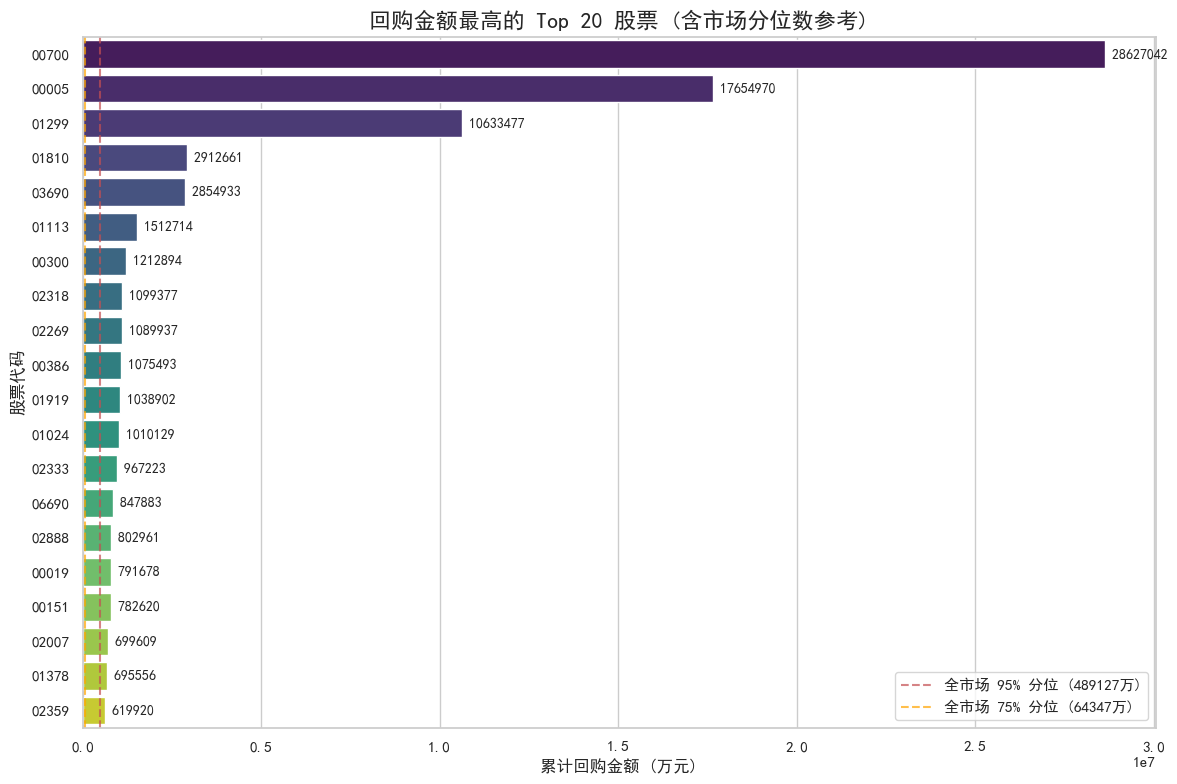
\includegraphics[width=0.95\textwidth]{1.png}
    \caption{样本期内累计回购金额最高的 Top 20 股票（含市场分位数参考）}
    \label{fig:buyback_cross}
    \vspace{0.2cm}
    \begin{flushleft}
        \footnotesize
        \textbf{说明：}横轴为样本期内累计实际回购金额（万元），纵轴为股票代码。虚线分别表示全市场回购金额的 75\% 与 95\% 分位数，用以刻画回购行为在截面上的集中程度。
    \end{flushleft}
\end{figure}

上述特征表明，实际回购数据在横截面与时间维度上均具有显著的非均质性，这一事实在后续回购变量构造与实证设定中需要被显式考虑。

\subsection{阶段性结论}

通过对东方财富实际回购数据的系统清洗与样本约束，本文构建了一个\textbf{日频、可量化、可与公告数据对齐}的港股实际回购数据库。初步描述性分析显示，实际回购行为在时间与截面两个维度上均表现出强烈的集中性与异质性，这进一步强化了从“公告条数”转向“行为强度”作为研究对象的必要性。

在下一节中，本文将基于该行为级回购数据，反向对照公告披露信息，具体分析公告数据的冗余性及其与真实回购行为之间的对应关系。




























% \section{公告—行为映射：以 700 与 2359 为例的对照分析}
% \subsection{从实际回购反查公告：700（腾讯）的案例链路}
% \subsection{公告冗余与类型差异：2359 案例与对比结论}
% \subsection{阶段性结论：公告 $\neq$ 事件，行为口径的必要性}


\section{从实际回购行为出发的公告映射探索}

\subsection{基于单一公司的回购行为刻画：以腾讯（00700）为例}

在完成对东财实际回购数据的初步清洗与整理后，本文首先选取腾讯控股（00700）作为案例公司，对其样本期内的实际回购行为进行深入观察。选择腾讯作为分析对象，主要基于其回购频率高、回购规模大且时间跨度长，有助于更清晰地刻画实际回购行为的动态特征。

基于清洗后的逐日回购金额数据，可以观察到，腾讯的回购行为并非零散发生，而是呈现出较为稳定且持续的时间结构：在若干连续交易日内，回购金额保持在相对集中的区间，形成明显的“回购窗口”。这一现象表明，实际回购更接近于一种阶段性、计划性执行的资本配置行为，而非完全随机或单日冲击式操作。

该结果为后续分析提供了一个重要事实基础：即在公司层面，实际回购行为本身已经蕴含了清晰的时间结构，这一结构未必能够被简单的公告事件所直接捕捉。

\subsection{从实际回购反向追溯公告：公告冗余与信息分散问题}

在明确腾讯实际回购行为的时间结构后，本文进一步尝试从“行为”反向出发，追溯与其对应的回购公告信息。具体而言，以已识别出的实际回购日期为锚点，向前后搜索相关公告记录，试图建立实际回购行为与公告披露之间的对应关系。

\begin{figure}[H]
    \centering
    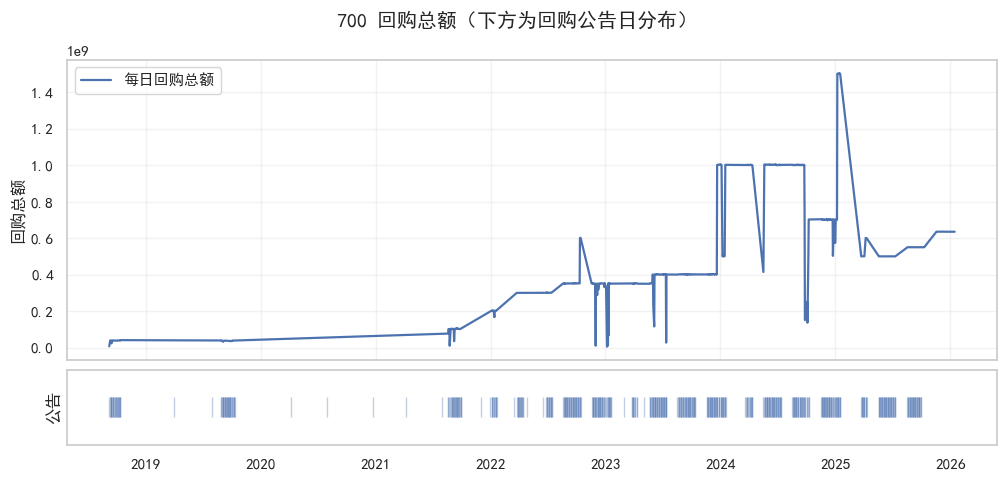
\includegraphics[width=0.95\textwidth]{2.png}
    \caption{腾讯（00700）实际回购行为与回购公告披露的时间对照}
    \label{fig:700_buyback_announce}
    \vspace{0.2cm}
    \begin{flushleft}
        \footnotesize
        \textbf{说明：}上图为腾讯逐日实际回购总金额的时间序列；下图为对应期间内回购相关公告的披露日期分布。可以观察到，实际回购行为呈现出明显的阶段性与连续性，而公告披露则表现为离散且密集的时间分布，两者之间不存在一一对应关系。
    \end{flushleft}
\end{figure}

分析结果显示，腾讯在样本期内的回购公告存在显著的冗余与重复特征：围绕同一轮回购执行，往往伴随多条内容高度相似、时间相近的公告记录。这些公告在标题、措辞及披露信息层面差异有限，但在数据层面却被记录为多个独立事件。

\begin{figure}[H]
    \centering
    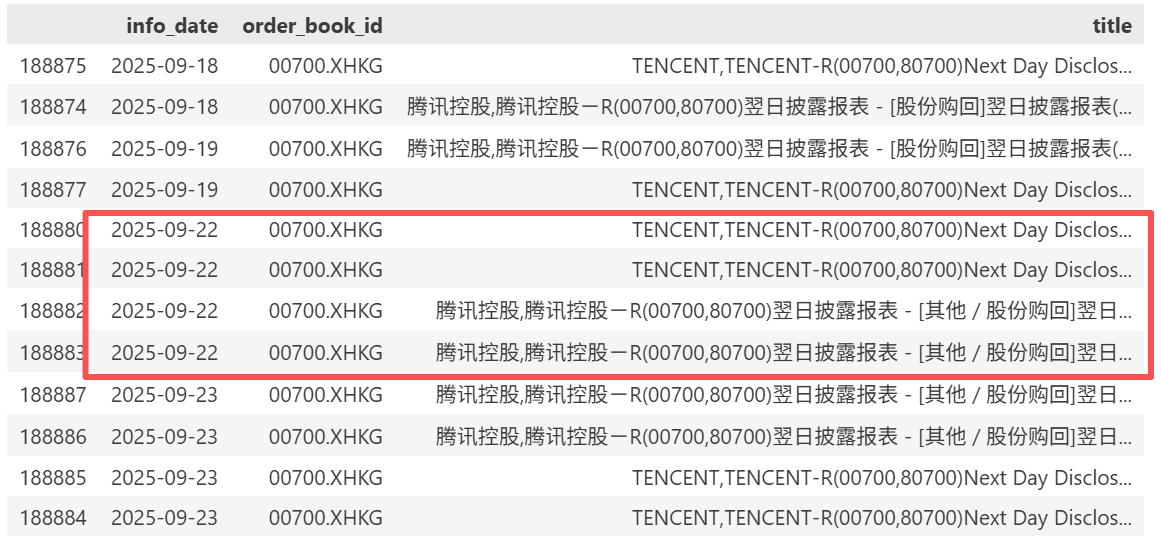
\includegraphics[width=0.95\textwidth]{3.png}
    \caption{腾讯（00700）回购公告在同一披露日的重复记录示例}
    \label{fig:700_duplicate_announcements}
    \vspace{0.2cm}
    \begin{flushleft}
        \footnotesize
        \textbf{说明：}图中展示了腾讯控股（00700）在同一披露日（2025-09-22）出现的多条回购相关公告记录。尽管这些公告在数据库中被视为独立事件，但其标题内容高度相似，实质上对应同一回购行为在不同披露口径或分类下的重复呈现。该现象表明，公告层面的“事件”并不等同于经济意义上的独立回购执行，有必要在后续分析中对公告进行去重与类型区分，以避免高估回购事件的发生频率。
    \end{flushleft}
\end{figure}


进一步清洗公告后发现，即便在去除高度重复的公告条目后，公告披露时间与实际回购执行时间之间仍然不存在一一对应关系。部分公告发生在实际回购执行之前，更多公告则滞后于回购行为发生，甚至在多个交易日后才完成披露。

这一发现表明，回购公告在信息传递层面存在显著的分散性与滞后性，使得单纯依赖公告事件来刻画回购行为，可能会引入严重的测度误差。


\subsection{外推至其他高回购公司：以药明康德（2359）为例}

为检验上述发现是否仅为腾讯个案特征，本文进一步将同一分析流程外推至另一家回购规模显著的公司——药明康德（2359）。该公司在样本期内的累计回购金额位于市场高分位区间，具有较强的代表性。

\begin{figure}[H]
    \centering
    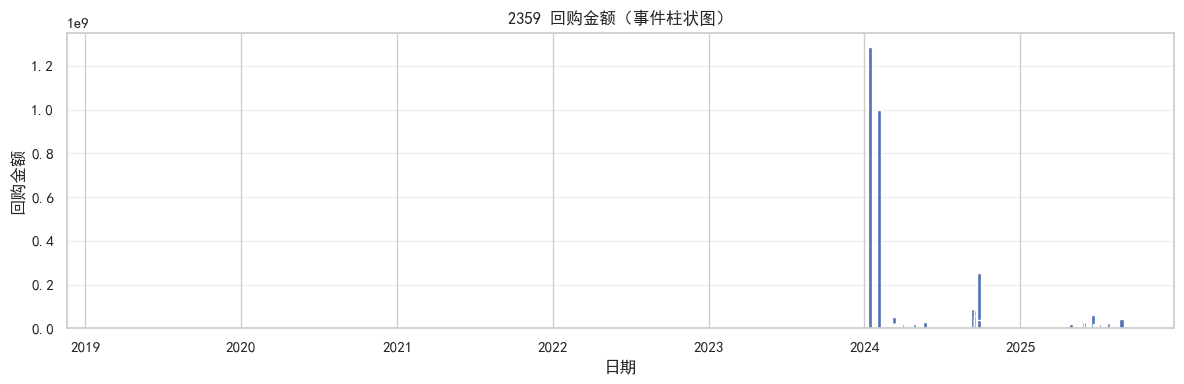
\includegraphics[width=0.95\textwidth]{4.png}
    \caption{药明康德（02359）实际回购金额的事件型分布}
    \label{fig:2359_buyback_event}
    \vspace{0.2cm}
    \begin{flushleft}
        \footnotesize
        \textbf{说明：}图中展示了药明康德（02359）逐日实际回购金额的时间分布。可以观察到，该公司的回购行为高度集中于少数交易日，呈现出明显的“事件型”特征，而非连续、多日执行的回购模式。这表明，不同公司在实际回购执行方式上存在显著异质性。
    \end{flushleft}
\end{figure}

分析结果显示，药明康德的实际回购行为同样呈现出明显的阶段性特征，其回购金额在若干时间窗口内集中发生。而在公告层面，该公司亦存在多种类型的回购相关公告，包括回购计划披露、执行进度更新及结果性公告等。

\begin{figure}[H]
    \centering
    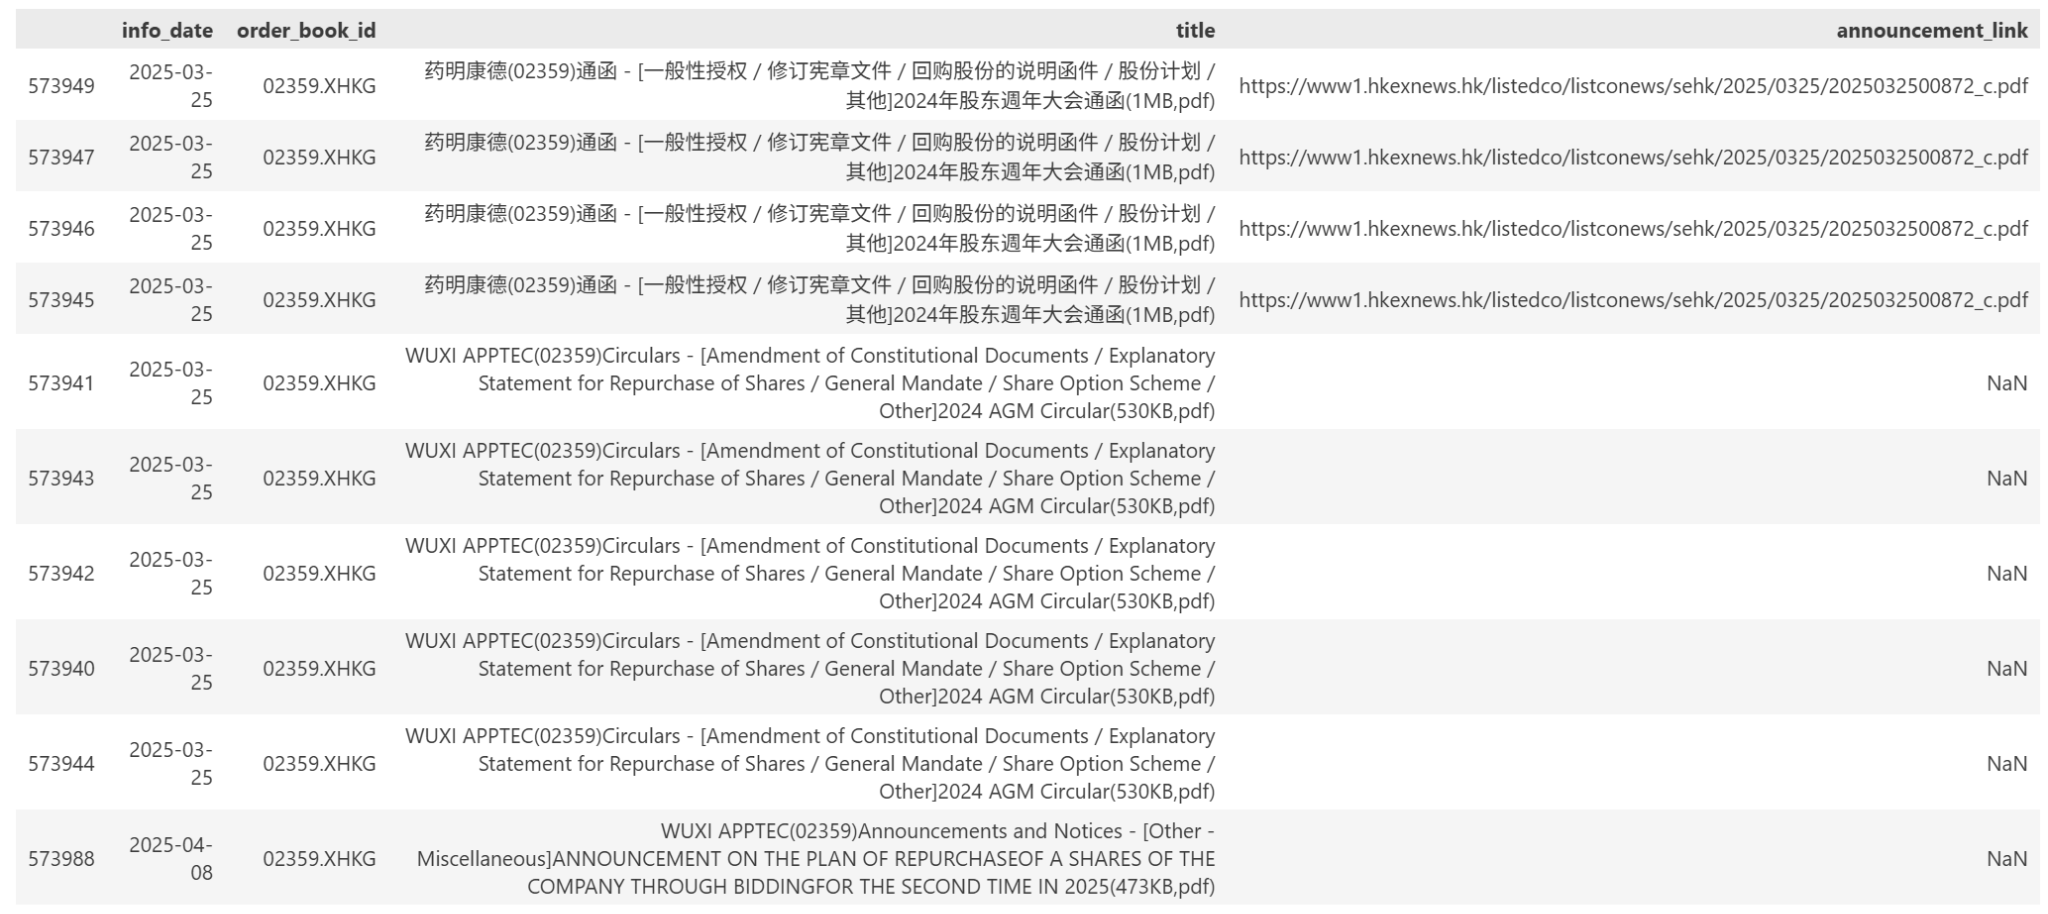
\includegraphics[width=0.95\textwidth]{5.png}
    \caption{药明康德（02359）回购相关公告在同一披露日的多重记录示例}
    \label{fig:2359_duplicate_announcements}
    \vspace{0.2cm}
    \begin{flushleft}
        \footnotesize
        \textbf{说明：}图中列示了药明康德（02359）在同一披露日（2025-03-25）出现的多条回购相关公告记录。尽管这些公告在数据库中被视为不同事件，其内容主要集中于回购授权、股东大会通函及回购计划说明等，实质上并不对应多个独立的回购执行行为。这一现象进一步表明，公告层面的事件数量无法直接代表真实回购行为的发生频率。
    \end{flushleft}
\end{figure}

更为重要的是，不同类型公告与实际回购执行之间的对应关系存在显著差异：部分公告更偏向于事前授权与计划说明，而另一些公告则更接近事后披露。这一结构性差异进一步强化了本文的核心认识——回购公告并非单一、同质的信息载体，而是包含多种经济含义不同的披露行为。



































% \section{方法论推进：公告类型再梳理与研究对象锁定}
% \subsection{两类主要公告行为的识别与分类规则草案}
% \subsection{去重/聚合口径的候选方案（按日、按窗口、按“行为”）}


\section{方法论推进：公告类型再梳理与研究对象锁定}

\subsection{回购公告类型的再划分与研究对象的锁定}

前文基于腾讯（00700）与药明康德（02359）的案例分析表明，港股回购相关公告在披露频率、内容结构及与实际回购行为的对应关系上均存在显著异质性。若不对公告类型进行进一步区分，而直接将所有回购相关公告视为同质事件用于实证分析，可能会引入较大的测度噪声，甚至掩盖真实的经济效应。

基于对公告标题、正文内容及披露时点的综合考察，本文将回购相关公告初步划分为以下几类：

\begin{itemize}
    \item \textbf{回购授权类公告}：主要包括一般性授权、股东大会通函及回购计划说明等，此类公告通常发生在回购执行之前，更多反映公司层面的制度性安排，而非具体回购行为；
    \item \textbf{回购执行类公告}：披露已发生的回购数量、价格或金额，具有明确的事后确认性质；
    \item \textbf{其他回购相关公告}：如制度修订、补充说明或与回购间接相关的披露，其经济含义相对模糊。
\end{itemize}

结合实际回购数据的时间结构可以发现，授权类公告在时间上往往早于或独立于回购执行，而执行类公告则普遍存在披露滞后，且在同一披露日内可能出现多条内容高度相似的重复公告。因此，无论是授权类还是执行类公告，均难以直接作为“回购行为发生当日”的精准代理。

在上述背景下，本文进一步注意到一类具有特殊时间结构的公告——\textbf{“翌日披露（Next Day Disclosure）”类回购公告}。该类公告通常在回购行为发生后的下一个交易日披露，其内容直接对应前一交易日已完成的回购执行，且披露逻辑相对规范，信息冗余程度显著低于其他类型公告。

从行为与披露的对应关系来看，翌日披露公告在时间上与实际回购执行最为接近，在信息含量上也更具针对性。因此，在后续实证分析中，本文将该类公告作为核心研究对象，用以刻画回购信息对市场价格的短期影响。

\subsection{“翌日披露”公告的识别规则}

为在公告层面进一步锁定与实际回购行为时间结构最为接近的信息披露，本文基于公告标题文本构建关键词匹配规则，对回购相关公告进行细分筛选。具体而言，本文在公告标题中识别包含“翌日 / 次日 / Next Day / the next day”等关键词的记录，并将其视为潜在的“翌日披露”类公告。

在此基础上，结合前文已识别的回购授权类与完成披露类关键词，本文将回购相关公告划分为以下互斥类别：
\begin{itemize}
    \item \textbf{mandate}：回购授权类公告，通常对应一般性授权或股东大会相关披露；
    \item \textbf{nextday\_only}：标题中明确包含“翌日披露”关键词，且不包含回购完成类表述的公告；
    \item \textbf{complete\_only}：回购完成或结果披露类公告，但未出现“翌日披露”关键词；
    \item \textbf{neither}：未能明确归入上述三类的其他回购相关公告。
\end{itemize}

该分类规则使得不同披露目的与时间属性的回购公告在数据层面得以区分，为后续实证分析中聚焦信息含量更为集中的公告类型提供了可操作的筛选标准。

\subsubsection{公告类型分布的初步统计}

基于上述规则对样本内回购相关公告进行分类后，不同类型公告在数量上呈现出显著差异。统计结果显示，“翌日披露”类公告在样本中占据主导地位，其数量明显高于回购授权类及完成披露类公告。

具体而言，在全部回购相关公告中，“nextday\_only” 类公告共计 26,222 条，显著高于回购授权类公告（4,291 条）与完成披露类公告（199 条）；此外，仍有少量公告（2,384 条）未能明确归入上述三类。

这一分布特征表明，“翌日披露”并非少数公司的特殊披露习惯，而是在港股回购信息披露中具有广泛代表性的公告形式。这也进一步支持本文在后续分析中，将该类公告作为核心研究对象，用以刻画回购信息的短期市场反应。

\begin{table}[H]
    \centering
    \caption{回购相关公告类型的数量分布}
    \label{tab:announcement_bucket_dist}
    \renewcommand{\arraystretch}{1.2}
    \begin{tabular}{l r}
        \toprule
        \textbf{公告类型（bucket）} & \textbf{公告数量} \\
        \midrule
        nextday\_only   & 26{,}222 \\
        mandate        & 4{,}291 \\
        complete\_only & 199 \\
        neither        & 2{,}384 \\
        \bottomrule
    \end{tabular}
    \vspace{0.2cm}
    \begin{flushleft}
        \footnotesize
        \textbf{说明：}表中统计了基于公告标题关键词规则划分的不同回购公告类型的样本数量。其中，“nextday\_only”类公告数量显著高于其他类型，表明“翌日披露”是港股回购信息披露中最为常见且具有代表性的形式。
    \end{flushleft}
\end{table}







































% \section{初步实证：聚焦“明日披露”公告的事件研究设计}
% \subsection{研究问题与识别思路（时间线与不前视约束）}
% \subsection{Y 的定义：$t{+}1$ 日收益与未来 5 日累计收益}
% \subsection{Welch-$t$ 检验设定与结果解读（当前版本）}
% \subsection{尚未解决的问题与下一步改进方向}

\section{基于“翌日披露”回购公告的初步实证分析}

\subsection{研究设计与事件定义}

基于前文对回购公告类型的系统梳理，本文在初步实证阶段聚焦于“翌日披露（Next Day Disclosure）”类回购公告。选择该类公告作为事件定义，主要基于以下考虑：其一，该类公告在时间结构上与实际回购行为最为接近；其二，相较授权类或完成披露类公告，其信息冗余程度显著较低；其三，该类公告在样本中具有较高的覆盖度，具备统计分析的可行性。

在事件定义上，本文将公告披露日记为事件日 $t=0$。需要强调的是，虽然该类公告披露的是前一交易日已发生的回购行为，但从市场参与者的信息集角度看，公告披露当日仍是回购信息首次被广泛、公开获取的时间点，因此将其作为事件日具有合理性。

\subsection{收益指标与事件窗口设定}

在收益变量的选取上，本文采用两类指标以刻画回购公告的短期市场反应。第一类为公告披露日后的单日收益（$t+1$ 日收益），用于衡量回购信息的即时价格反应；第二类为公告披露日后若干交易日内的累计收益（如未来 5 个交易日累计收益），以捕捉可能存在的短期持续效应。

对应地，本文关注的核心事件窗口包括：
\begin{itemize}
    \item $[0, +1]$：公告披露日至次一交易日；
    \item $[0, +5]$：公告披露日至未来 5 个交易日的累计区间。
\end{itemize}

该设定兼顾了信息反应的及时性与可能存在的延迟消化效应，适合作为初步实证检验的观察窗口。


\subsection{实证方法：Welch t 检验}

为检验回购公告事件日前后收益是否存在显著差异，本文采用 Welch t 检验（Welch's t-test）对事件相关收益进行统计检验。相较于传统的两样本 t 检验，Welch t 检验不要求两组样本具有相同方差，更适合用于金融收益这类波动性异质且分布特征不稳定的数据。

具体而言，本文将事件样本中公告披露后的收益分布，与对应的基准收益分布进行比较，检验两者在均值层面是否存在统计显著差异。该方法旨在回答一个基础但关键的问题：在“翌日披露”类回购公告出现后，股票收益是否在统计意义上偏离其常态水平。


\subsection{初步结果与现象描述}

\begin{table}[H]
    \centering
    \caption{“翌日披露”回购公告的事件日与非事件日收益对比（Welch t 检验）}
    \label{tab:welch_event_vs_nonevent}
    \renewcommand{\arraystretch}{1.2}
    \begin{tabular}{l r r r r r r}
        \toprule
        \textbf{收益指标} & 
        \textbf{事件日均值} & 
        \textbf{非事件日均值} & 
        \textbf{差值} & 
        \textbf{t 统计量} & 
        \textbf{事件样本数} & 
        \textbf{非事件样本数} \\
        \midrule
        $r_{t+1}$ & 
        0.001609 & 
        0.000161 & 
        0.001448 & 
        7.84 & 
        26{,}186 & 
        624{,}993 \\
        $r_{t+1:t+5}$ & 
        0.002674 & 
        -0.001347 & 
        0.004022 & 
        9.82 & 
        26{,}106 & 
        624{,}122 \\
        \bottomrule
    \end{tabular}
    \vspace{0.2cm}
    \begin{flushleft}
        \footnotesize
        \textbf{说明：}表中比较了“翌日披露”回购公告发生后的收益，与非事件日收益的均值差异。采用 Welch t 检验以允许事件日与非事件日收益具有不同方差。结果显示，事件日后的短期收益在均值层面显著高于非事件日。
    \end{flushleft}
\end{table}

\begin{table}[H]
    \centering
    \caption{回购公告事件日前后逐日平均收益与累计收益}
    \label{tab:event_time_path}
    \renewcommand{\arraystretch}{1.2}
    \begin{tabular}{r r r}
        \toprule
        \textbf{相对事件日} & 
        \textbf{当日平均收益} & 
        \textbf{累计平均收益} \\
        \midrule
        $-5$ & -0.000787 & -0.000787 \\
        $-4$ & -0.001225 & -0.002013 \\
        $-3$ & -0.001380 & -0.003393 \\
        $-2$ & -0.001721 & -0.005114 \\
        $-1$ & -0.002368 & -0.007481 \\
        $0$  & -0.001889 & -0.009370 \\
        $+1$ &  0.001300 & -0.008070 \\
        $+2$ &  0.000596 & -0.007474 \\
        $+3$ &  0.000225 & -0.007249 \\
        $+4$ &  0.000234 & -0.007015 \\
        $+5$ &  0.000144 & -0.006871 \\
        \bottomrule
    \end{tabular}
    \vspace{0.2cm}
    \begin{flushleft}
        \footnotesize
        \textbf{说明：}表中报告了以“翌日披露”回购公告为事件日的相对时间收益路径。事件日前累计收益呈持续下降趋势，而事件日后平均收益转为正值，显示回购信息披露可能对应价格路径的阶段性反转。
    \end{flushleft}
\end{table}

\begin{figure}[H]
    \centering
    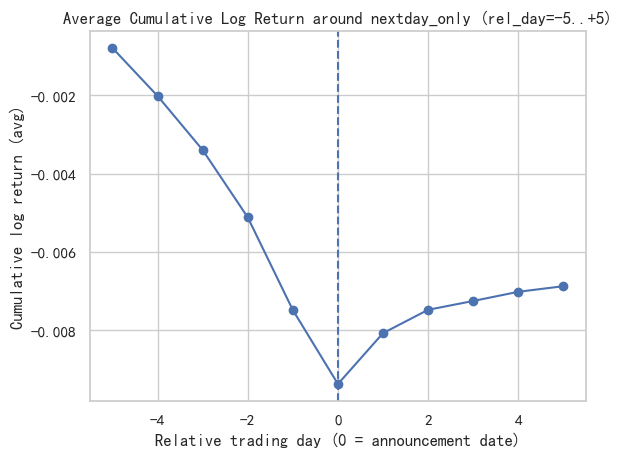
\includegraphics[width=0.8\textwidth]{6.png}
    \caption{“翌日披露”回购公告前后的平均累计对数收益路径}
    \label{fig:cumlogret_nextday}
    \vspace{0.2cm}
    \begin{flushleft}
        \footnotesize
        \textbf{说明：}图中展示了以“翌日披露”回购公告为事件日的平均累计对数收益路径，事件窗口为 $[-5,+5]$。虚线表示公告披露日（$t=0$）。可以观察到，公告前累计收益呈持续下降趋势，而公告后收益路径逐步回升，表明回购信息披露可能对应价格路径的阶段性修正。
    \end{flushleft}
\end{figure}


初步实证结果显示，在以“翌日披露”回购公告为事件定义的样本中，公告披露后短期收益在均值层面呈现出一定程度的正向偏移，但该效应在不同事件窗口下的显著性并不稳定。

在 $t+1$ 日收益层面，部分样本中观察到公告后收益相较基准存在正向变化，但整体统计显著性有限；在 $[0,+5]$ 的累计收益窗口中，收益分布的离散程度有所上升，显示回购信息的市场反应可能存在较强的异质性。

上述结果表明，尽管“翌日披露”类回购公告在信息结构上相对干净，但其对应的市场反应并非简单、统一的正向冲击。这一现象提示，回购公告的价格效应可能依赖于更丰富的条件因素，如回购规模、公司特征或市场状态等。


\subsection{阶段性小结与未解问题}

\begin{table}[H]
    \centering
    \caption{不同事件窗口内的平均累计收益及显著性检验}
    \label{tab:event_window_test}
    \renewcommand{\arraystretch}{1.2}
    \begin{tabular}{l r r r}
        \toprule
        \textbf{事件窗口} & 
        \textbf{平均累计收益} & 
        \textbf{t 统计量} & 
        \textbf{事件数} \\
        \midrule
        $[-5,-1]$（公告前） & -0.007481 & -18.27 & 26{,}205 \\
        $[0,+1]$（公告期）  & -0.000590 & -2.35  & 26{,}205 \\
        $[+1,+5]$（公告后） &  0.002497 &  6.01  & 26{,}186 \\
        \bottomrule
    \end{tabular}
    \vspace{0.2cm}
    \begin{flushleft}
        \footnotesize
        \textbf{说明：}表中报告了不同事件窗口内的平均累计对数收益，并对其是否显著偏离零进行 t 检验。结果显示，回购公告前存在显著负收益，而公告后窗口内收益显著为正，表明回购信息可能对应价格路径的阶段性修正。
    \end{flushleft}
\end{table}


综上所述，本文在严格筛选回购公告类型的基础上，对“翌日披露”类回购公告进行了初步的事件型实证分析。结果显示，该类公告在短期内可能伴随一定的正向收益反应，但整体效应尚不稳定，且存在显著的样本异质性。

这意味着，单纯依赖公告事件本身，仍难以充分刻画回购行为的市场影响。后续研究有必要进一步引入回购强度、回购持续性及公司基本面特征等维度，对回购信息的价格效应进行更细致的刻画与分组分析。






\section{股东回报因子的统一衰减建模框架}

在前文的实证分析中，本文已经从公告层面与实际行为层面，验证了港股市场中回购相关信息在短期内具有一定的价格影响。然而，事件研究本身更多刻画的是局部、离散的市场反应，而无法直接用于构建连续、可交易的量化因子。因此，有必要进一步回答一个更为根本的问题：如何将分红、回购等离散发生的公司行为，系统性地转化为能够反映公司长期股东回报能力的连续信号。

基于这一动机，本节在总回报模型（Total Payout Model）的思想框架下，构建统一的股东回报信号，并引入信息衰减机制，将原始的、稀疏的回报事件转化为平滑、可累积的因子序列。该框架不仅能够容纳回购行为，也为后续将回购信息与其他回报形式进行统一建模提供了基础。

\subsection{原始总回报信号（Raw Total Yield Signal）}

本文将公司在单个交易日内对股东产生的回报行为，统一表示为当日的瞬时收益率信号 $S_{\text{raw},t}$。该信号的经济含义在于：若投资者在 $t$ 日持有该股票，则由于公司层面的回报行为（包括分红、回购及偿债）所获得的理论收益率。

形式化地，原始总回报信号定义为：
\begin{equation}
S_{\text{raw},t}
=
\frac{Div_t}{M_t}
+
\alpha \cdot \frac{Buyback_t}{M_t}
+
\beta \cdot \frac{\max(0,-\Delta Debt_t)}{M_t},
\end{equation}
其中，$M_t$ 表示股票在 $t$ 日收盘时的总市值，用于对不同规模公司的回报行为进行标准化处理。$Div_t$ 表示当日分红金额，若 $t$ 日为除息日，则为当次分红总额，否则为零；$Buyback_t$ 表示公司在 $t$ 日实际发生的回购耗资总额；$\Delta Debt_t$ 表示公司净债务的日度变化。

系数 $\alpha$ 与 $\beta$ 用于控制回购与偿债是否纳入总回报信号的计算。在后续分析中，本文将以分红作为基础的回报形式，并将回购与偿债视为可选的补充回报渠道，从而考察不同回报定义下因子表现的稳健性。

\subsection{信息衰减模型与因子合成的基本思想}

需要指出的是，$S_{\text{raw},t}$ 本身具有明显的“脉冲型”特征：在大多数交易日内，该信号为零，而在发生分红或回购时出现显著跳跃。若直接将该信号作为因子使用，将导致因子序列过于稀疏，难以刻画市场对回报信息的持续反应。

因此，本文引入信息衰减（Information Decay）的思想，假定市场对公司回报行为的认知并非在单日内完全消化，而是随着时间推移或交易活动的进行逐步衰减。通过将原始回报信号与衰减机制相结合，可以将离散事件转化为连续、可积累的因子序列。

在具体实现上，本文从两个互补的维度刻画信息衰减过程：一是基于日历时间的衰减，二是基于交易活跃度的衰减。

\subsection{基于 IC 衰减的参数标定}

为定量刻画信息衰减速度，本文采用事件研究的方法，考察原始回报信号 $S_{\text{raw}}$ 的预测能力（Information Coefficient, IC）随时间推移的变化规律。具体而言，计算信号与未来 $k$ 日超额收益之间的相关系数，并观察其随 $k$ 增大的衰减情况。

假设 IC 随时间呈指数衰减，其函数形式设定为：
\begin{equation}
IC_{\text{time}}(k) = A \cdot e^{-\lambda_{\text{time}} k} + \varepsilon_k.
\end{equation}
通过对上述函数进行非线性最小二乘估计，可以得到时间维度的信息衰减速率 $\lambda_{\text{time}}$。该参数反映了回报信息在日历时间上的边际有效性递减速度，是后续因子合成的重要输入。

\subsection{交易维度的信息衰减建模}

除时间维度外，交易行为本身也是信息消化的重要渠道。大量交易往往意味着投资者对信息的重新定价，从而加速原有信息的失效。基于这一认识，本文引入累计换手率（Cumulative Turnover）作为交易维度的信息衰减刻画变量。

设 $x$ 表示自信号发生以来的累计换手率，则交易维度的 IC 衰减形式定义为：
\begin{equation}
IC_{\text{vol}}(x) = B \cdot e^{-\lambda_{\text{vol}} x} + \varepsilon_x.
\end{equation}
其中，$\lambda_{\text{vol}}$ 描述单位换手率对信息衰减的影响强度。该参数刻画了交易活动在多大程度上加速市场对回报信息的吸收。

\subsection{因子合成模型一：按物理时间衰减}

基于估计得到的 $\lambda_{\text{time}}$，本文构建按日历时间衰减的连续股东回报因子 $Factor_{\text{time},t}$。首先定义单日时间衰减因子为：
\begin{equation}
\delta_{\text{time}} = e^{-\lambda_{\text{time}}}.
\end{equation}
在此基础上，因子采用递归方式进行更新，其计算公式为：
\begin{equation}
Factor_{\text{time},t}
=
Factor_{\text{time},t-1} \cdot \delta_{\text{time}}
+
S_{\text{raw},t}.
\end{equation}
该形式表明，历史回报信息将随着时间推移按固定比例衰减，而新的回报事件则被即时纳入因子之中。

\subsection{因子合成模型二：按交易量衰减}

与时间衰减模型不同，交易量衰减模型允许信息衰减速度随市场活跃度动态变化。设 $Turnover_t$ 为 $t$ 日的换手率，则当日的交易衰减因子定义为：
\begin{equation}
\delta_{\text{vol},t} = e^{-\lambda_{\text{vol}} \cdot Turnover_t}.
\end{equation}
相应地，交易量衰减因子的递推公式为：
\begin{equation}
Factor_{\text{vol},t}
=
Factor_{\text{vol},t-1} \cdot \delta_{\text{vol},t}
+
S_{\text{raw},t}.
\end{equation}
该模型允许在高换手时期更快地削弱历史信息权重，从而更贴近市场实际的信息更新过程。

\subsection{实物分红（Script Dividends）的估值处理}

港股市场中普遍存在以实物分红替代现金分红的情况。若忽略该类分红形式，将导致股东回报信号的系统性低估。为此，本文对实物分红采用统一的等价现金化处理方法。

具体而言，将实物分红折算为等效的每股现金分红：
\begin{equation}
V_{\text{script}} = \frac{P_{\text{distributed}}}{N_{\text{basis}}},
\end{equation}
其对应的分红收益率为：
\begin{equation}
Yield_{\text{script}}
=
\frac{V_{\text{script}}}{P_{\text{current}}}
=
\frac{P_{\text{distributed}}}{N_{\text{basis}} \cdot P_{\text{current}}}.
\end{equation}
其中，$P_{\text{distributed}}$ 表示除权日被分派资产的收盘价，$N_{\text{basis}}$ 为分派基数，$P_{\text{current}}$ 为除权日股票的收盘价。通过上述处理，可以将实物分红与现金分红在收益率层面进行统一刻画。




\section{本期小结与下期计划}

\subsection{本期结论}

\begin{itemize}
    \item 港股市场中回购公告在数量与时间维度上存在显著冗余，同一回购行为往往对应多次公告披露，公告条数本身并不能直接刻画回购强度或经济含义。
    
    \item 基于东财逐日数据观察到的实际回购行为呈现出明显的阶段性与连续性特征，与公告披露的离散分布形成鲜明对比，验证了“公告 $\neq$ 行为”的核心判断。
    
    \item 个股案例分析（如腾讯、药明康德）表明，头部公司回购金额在全市场分布中高度集中，其回购行为在时间与规模上均具有显著异质性。
    
    \item “翌日披露”类回购公告在港股公告体系中占据主导地位，且围绕该类事件的未来收益在统计上呈现出显著差异，说明该类公告具有一定的信息含量。
    
    \item 初步事件研究结果显示，回购相关信息的价格反应并非完全在公告当日消化，存在跨期效应，为后续引入信息衰减建模提供了经验证据。
\end{itemize}


\subsection{下期计划}

\begin{itemize}
    \item \textbf{数据层面：}\\
    在现有逐日实际回购数据与公告数据基础上，进一步完善公告类型标签体系，重点区分授权类、执行类与进度披露类回购公告，并探索将公告信息与实际回购金额进行更精细的对齐与聚合。

    \item \textbf{方法层面：}\\
    在事件研究结果的基础上，引入信息衰减思想，探索将离散回购事件映射为连续日频信号的建模方式，包括基于时间窗口与记忆衰减的回购强度指标构造。

    \item \textbf{实证层面：}\\
    将构建的回购相关日频信号纳入统一的股东回报因子框架中，与分红等其他回报形式结合，系统检验其在未来收益预测中的有效性及稳健性。
\end{itemize}







\end{document}
